% !TEX root = BioInspired.tex

\chapter{Latex}
Big ole grab bag of latex sample code ....


\section{Some \LaTeX\ }

See Figure~\ref{systemdiagram}.  This is a floating
figure environment.  \LaTeX\ will try to put it close to where it was
typeset but will not allow the figure to be split if moving it can not
happen.  Figures, tables, algorithms and many other floating
environments are automatically numbered and placed in the appropriate
type of table of contents.  You can move these and the numbers will
update correctly.

\begin{figure}[tbh]
\begin{center}
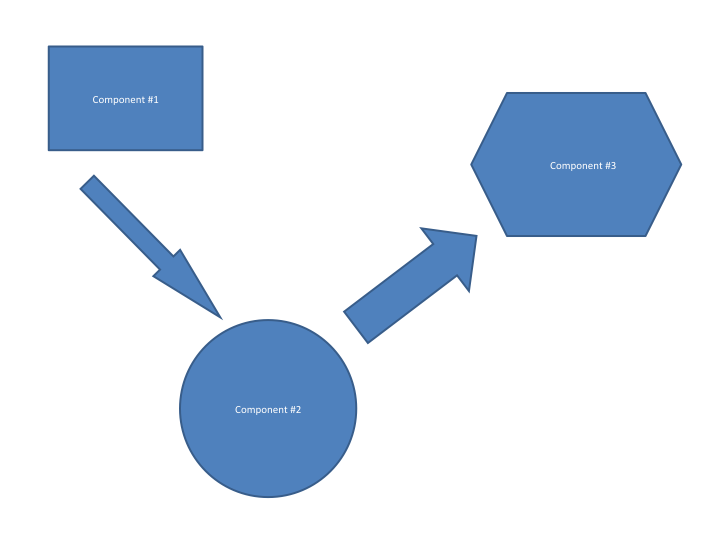
\includegraphics[width=0.75\textwidth]{./diagram}
\end{center}
\caption{A sample figure .... System Diagram \label{systemdiagram}}
\end{figure}




See Table~\ref{somenumbers}.  This is a floating table environment.
\LaTeX\ will try to put it close to where it was typeset but will not
allow the table to be split.

\begin{table}[tbh]
\caption{A sample Table ... some numbers. \label{somenumbers}}
\begin{center}
\begin{tabular}{|r|l|}
  \hline
  7C0 & hexadecimal \\
  3700 & octal \\ \cline{2-2}
  11111000000 & binary \\
  \hline \hline
  1984 & decimal \\
  \hline
\end{tabular}
\end{center}
\end{table}

Sample bullet list environment:
\begin{itemize}
\item According to the all knowing wikipedia, C is an all purpose imperative programming language.   
\item Developed between 1969 and 1973 by Dennis Ritchie.  [With help from Ken Thompson.]
\item One of the most influential computer languages.
\end{itemize}

Sample numbered list:
 \begin{enumerate}
 \item Predictor:  Small step in direction $\lambda \in {\cal N}(J_G(x))$:
\item Corrector:  $y^{k+1} = y^k + (J_G(y^k))^{-1}G(y^k,\lambda)$
\end{enumerate}

\section{Section\#1 }

Example Section.

\subsection{Subsection \#1}

Example subsection.

\subsubsection{Subsubsection \#1}

Because I can.   [But I did not assign a color to the font.]


\begin{equation}
\displaystyle\frac{\partial u}{\partial t} = k \left( \frac{\partial^2 u}{\partial x^2} +  \frac{\partial^2 u}{\partial y^2} \right)
\end{equation}

\subsection{Code Details}
Here is an example code listing:
\begin{lstlisting}
#include <stdio.h>
#define N 10
/* Block
 * comment */
 
int main()
{
    int i;
 
    // Line comment.
    puts("Hello world!");
 
    for (i = 0; i < N; i++)
    {
        puts("LaTeX is also great for programmers!");
    }
 
    return 0;
}
\end{lstlisting}
This code listing is not floating or automatically numbered.  If you want auto-numbering, but it in the algorithm environment (not algorithmic however) shown above.


Sample algorithm:  Algorithm~\ref{alg1}.  This algorithm environment is automatically placed - meaning it floats.   You don't have to worry about placement or numbering.  

\begin{algorithm} [tbh]                     % enter the algorithm environment
\caption{Calculate $y = x^n$}          % give the algorithm a caption
\label{alg1}                           % and a label for \ref{} commands later in the document
\begin{algorithmic}                    % enter the algorithmic environment
    \REQUIRE $n \geq 0 \vee x \neq 0$
    \ENSURE $y = x^n$
    \STATE $y \Leftarrow 1$
    \IF{$n < 0$}
        \STATE $X \Leftarrow 1 / x$
        \STATE $N \Leftarrow -n$
    \ELSE
        \STATE $X \Leftarrow x$
        \STATE $N \Leftarrow n$
    \ENDIF
    \WHILE{$N \neq 0$}
        \IF{$N$ is even}
            \STATE $X \Leftarrow X \times X$
            \STATE $N \Leftarrow N / 2$
        \ELSE[$N$ is odd]
            \STATE $y \Leftarrow y \times X$
            \STATE $N \Leftarrow N - 1$
        \ENDIF
    \ENDWHILE
\end{algorithmic}
\end{algorithm}
Citations look like~\cite{Choset:2005:PRM, arkin2009governing, lavalle2006}  and~\cite{wiki:asimo,lumelsky:1987, nolfi2000evolutionary}.  These are done automatically.  Just fill in the database {\tt designrefs.bib} using the same field structure as the other entries.  Then pdflatex the document, bibtex the document and pdflatex twice again.  The first pdflatex creates requests for bibliography entries.
The bibtex extracts and formats the requested entries.  The next pdflatex puts them in order and assigns labels.  The final pdflatex replaces references in the text with the assigned labels.
The bibliography is automatically constructed.  

\section{Section \#2}

An example of a minipage environment (gets side by side content - like two column mode).  Also there is an example of a flow chart using tikz.  
\noindent
Flowcharts\\[3mm]
\tikzstyle{startstop} = [rectangle, rounded corners, minimum width=3cm, minimum height=1cm,text centered, draw=black, fill=red!30]\tikzstyle{io} = [trapezium, trapezium left angle=70, trapezium right angle=110, minimum width=3cm, minimum height=1cm, text centered, draw=black, fill=blue!30]
\tikzstyle{process} = [rectangle, minimum width=3cm, minimum height=1cm, text centered, draw=black, fill=orange!30]
\tikzstyle{decision} = [diamond, minimum width=3cm, minimum height=1cm, text centered, draw=black, fill=green!30]
\tikzstyle{arrow} = [thick,->,>=stealth]
\begin{minipage}{0.45\textwidth}
\begin{tikzpicture}[node distance=2cm]
\node (start) [startstop] {Start};
\node (in1) [io, below of=start] {Input};
\node (pro1) [process, below of=in1] {Process 1};
\node (dec1) [decision, below of=pro1] {Decision 1};
\end{tikzpicture}\\
\begin{picture}(0,0)
\put(0,0){Flow:   \vector(1,0){40}}
\end{picture}
\end{minipage}
\begin{minipage}{0.45\textwidth}
\begin{tikzpicture}[node distance=2cm]
\node (start) [startstop] {Start};
\node (in1) [io, below of=start] {Input};
\node (pro1) [process, below of=in1] {Process 1};
\node (dec1) [decision, below of=pro1, yshift=-0.5cm] {Decision 1};
\node (pro2a) [process, below of=dec1, yshift=-0.5cm] {Process 2a};
\node (pro2b) [process, right of=dec1, xshift=2cm] {Process 2b};
\node (out1) [io, below of=pro2a] {Output};
\node (stop) [startstop, below of=out1] {Stop};
\draw [arrow] (start) -- (in1);
\draw [arrow] (in1) -- (pro1);
\draw [arrow] (pro1) -- (dec1);
\draw [arrow] (dec1) -- (pro2a);
\draw [arrow] (dec1) -- (pro2b);
\draw [arrow] (dec1) -- node[anchor=east] {yes} (pro2a);
\draw [arrow] (dec1) -- node[anchor=south] {no} (pro2b);
\draw [arrow] (pro2b) |- (pro1);
\draw [arrow] (pro2a) -- (out1);
\draw [arrow] (out1) -- (stop);
\end{tikzpicture}
\end{minipage}



More in the sample document at the end.
